% Шаблон для оформления работ в ВШЭ
% Используется xelatex

\documentclass[a4paper,10pt]{article}

%%% Работа с русским языком
\usepackage[utf8]{inputenc}		% кодировка исходного текста
\usepackage[T2A]{fontenc}			% кодировка
\usepackage{cmap}					% поиск в PDF
\usepackage{mathtext} 				% русские буквы в формулах
\usepackage[english,russian]{babel}	% локализация и переносы

%%% Дополнительная работа с математикой
\usepackage{amsmath,amsfonts,amssymb,amsthm,mathtools} % AMS
\usepackage{icomma} % "Умная" запятая: $0,2$ --- число, $0, 2$ --- перечисление


%%% Рисунки
\usepackage[format=plain,
            font={small,it},
            figurename=Рисунок,
            figurewithin=section,
            labelsep=endash % Разделитель между числом и подписью (--)
            ]{caption}

%%% Заголовки
\usepackage{titlesec}
\renewcommand{\numberline}[1]{#1~}
\titleformat{\section}[block]{\fontsize{16}{12}\selectfont\bfseries\filcenter}{\thesection}{4pt}{}
\titleformat{\subsection}[block]{\fontsize{14}{12}\bfseries\filcenter}{\thesubsection}{4pt}{}
% \renewcommand{\thesection}{Глава \arabic{section} --}
% \renewcommand{\thesubsection}{\arabic{section}.\arabic{subsection} --}


\titlespacing*{\section}
{0pt}{0pt}{12pt} % left, top, bottom
\newcommand{\sectionbreak}{\clearpage}

\titlespacing*{\subsection}
{0pt}{12pt}{6pt}

%%% Оглавление
\usepackage{tocloft}
\renewcommand{\cftsecleader}{\cftdotfill{\cftdotsep}} % точки в оглавлении
\renewcommand\cfttoctitlefont{\hfill\Large\bfseries} % заголовок оглавления по центру
\renewcommand\cftaftertoctitle{\hfill\mbox{}} % продолжение заголовок по центру


%%% Работа с картинками
\usepackage{graphicx}  % Для вставки рисунков
\graphicspath{{diagrams/}{images/}{images2/}}  % папки с картинками
\setlength\fboxsep{3pt} % Отступ рамки \fbox{} от рисунка
\setlength\fboxrule{1pt} % Толщина линий рамки \fbox{}
\usepackage{wrapfig} % Обтекание рисунков текстом

%%% Работа с таблицами
\usepackage{array,tabularx,tabulary,booktabs} % Дополнительная работа с таблицами
\usepackage{longtable}  % Длинные таблицы
\usepackage{multirow} % Слияние строк в таблице

\newtheorem*{nonum}{Решение}

%%% Страница
\usepackage[fontsize=13pt]{scrextend}
\usepackage{geometry} % Простой способ задавать поля
	\geometry{top=20mm}
	\geometry{bottom=20mm}
	\geometry{left=30mm}
	\geometry{right=15mm}

\usepackage{setspace} % Интерлиньяж 1.5
    \onehalfspacing

\usepackage{paralist} % междустрочные отступы в списках

\usepackage{indentfirst} % Абзацные отступы
    \setlength{\parindent}{1.25cm}


\usepackage[normalem]{ulem} % для подчёркиваний uline
    \ULdepth = 0.2em % расстояние от линии до текста выше/ниже


\usepackage{fontspec}
    \setmainfont{Times New Roman}


\begin{document} % конец преамбулы, начало документа

\thispagestyle{empty}
\begin{center}
    \begingroup
    \fontsize{13pt}{15pt}\selectfont

    Пермский филиал федерального государственного автономного \\
    образовательного учреждения высшего образования \\
    <<Национальный исследовательский университет \\
    <<Высшая школа экономики>>

	\vspace{2em}
    \textit{Факультет экономики, менеджмента и бизнес-информатики}

    \vspace{4em}
    Бочкарев Вадим Александрович

    \vspace{3em}
    \textbf{АНАЛИЗ СЦЕНАРИЕВ ПРЕДМЕТНОЙ ОБЛАСТИ}

    \vspace{0.5em}
    \textit{Отчёт по лабораторной работе}

    \vspace{3em}

\fontsize{13pt}{15pt}\selectfont
    студента образовательной программы бакалавриата <<Программная инженерия>>\\
    по направлению подготовки \textit{\uline{09.03.04 Программная инженерия}}

\vfill

\hfill % заполнить пустоту по ширине
\parbox{6cm}{

    \fontsize{13pt}{15pt}\selectfont
    \begin{flushleft}
            Руководитель\\
            преподаватель кафедры\\
            информационных технологий в бизнесе

            \hrulefill

            В.П. Куприн
    \end{flushleft}
}

\vfill

\endgroup
\center{Пермь, 2021}\end{center}\newpage


\tableofcontents
\clearpage

\section*{Введение}\label{Введение}

В данном проекте проведём анализ сценариев предметной области в рамках
взаимодействия нескольких слоёв приложения.

\section{Анализ сценариев предметной области} \label{Анализ сценариев предметной области}

Поскольку планируется, что взаимодействие с приложением будет происходить
с помощью API по протоколу HTTP(s), то на диаграммах необходимо будет обозначить
следующие слои приложения:

\begin{asparaenum}
    \item Слой клиента: это может быть любое приложение, способное отправлять HTTP(s) запросы.
    \item Слой API: слой, который будет обрабатывать пришедшие со стороны клиента запросы.
        Этот слой будет обращаться к хранилищу конфигураций машин состояний (далее --- МС) и
        решать, какие изменения должны произойти.
    \item Слой хранилища конфигураций: слой представляет собой некую БД, в которой
        будут храниться конфигурации МС (настройки жизненного цикла, описания типа
        обрабатываемого объекта, текущее состояние объекта).
\end{asparaenum}

При создании МС клиент получает её уникальный идентификатор --- токен, который
будет необходим для совершения операций с ней. Токен представляет собой последовательность
случайных алфавитных и цифровых символов. Предполагается, что случайный перебор
токенов для получения доступа к чужой МС будет слишком времязатратным (это
будет обеспечено огромным числом возможных комбинаций токена).

\begin{figure}[htpb]
    \centering
    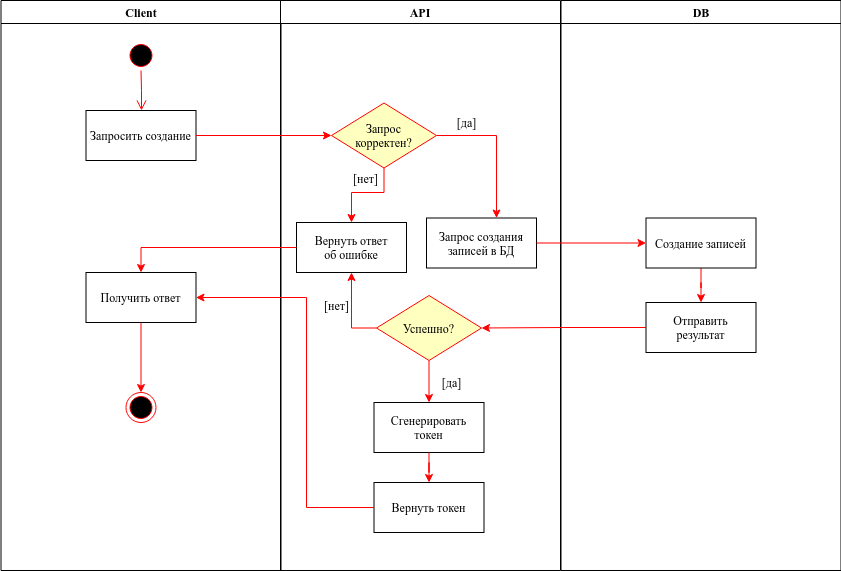
\includegraphics[width=0.8\textwidth]{activity_diagram}
    \caption{Диаграмма Activity создания}
    \label{fig:activity_diagram}
\end{figure}

<<Общение>> клиента с системой будет происходить с помощью формата данных JSON.
С помощью него будут закодированы все запросы и ответы.

Поскольку, в целом, взвзаимодействие с системой с точки зрения диаграммы activity,
то построим одну диаграмму для процесса создания МС.

% можно подумать насчёт HTTP кодов ответов при обращении к апи
Полученная диаграмма представлена на Рисунке~\ref{fig:activity_diagram}.

Диаграмма процесса получения состояния представлена на Рисунке~\ref{fig:activity_get_state}.

\begin{figure}[htpb]
    \centering
    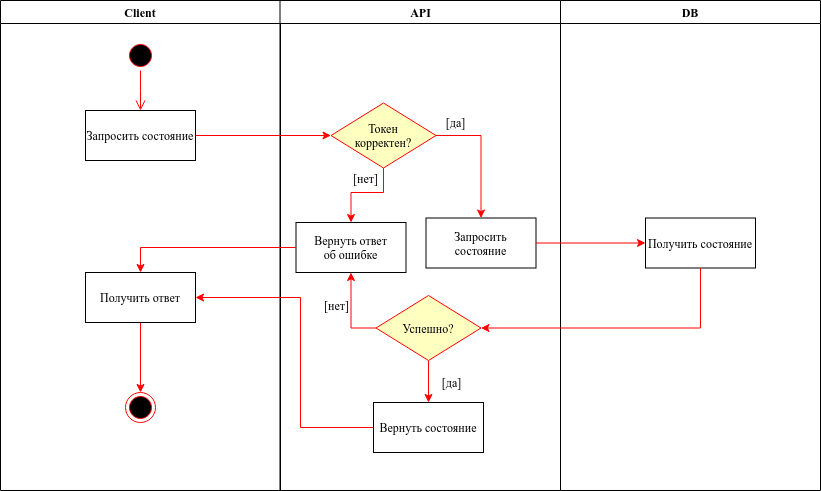
\includegraphics[width=0.8\textwidth]{diagrams/activity_get_state.png}
    \caption{Диаграмма Activity получения состояния}
    \label{fig:activity_get_state}
\end{figure}

Диаграмма процесса передачи изменения состояния представлена на Рисунке~\ref{fig:activity_send_change}.

\begin{figure}[htpb]
    \centering
    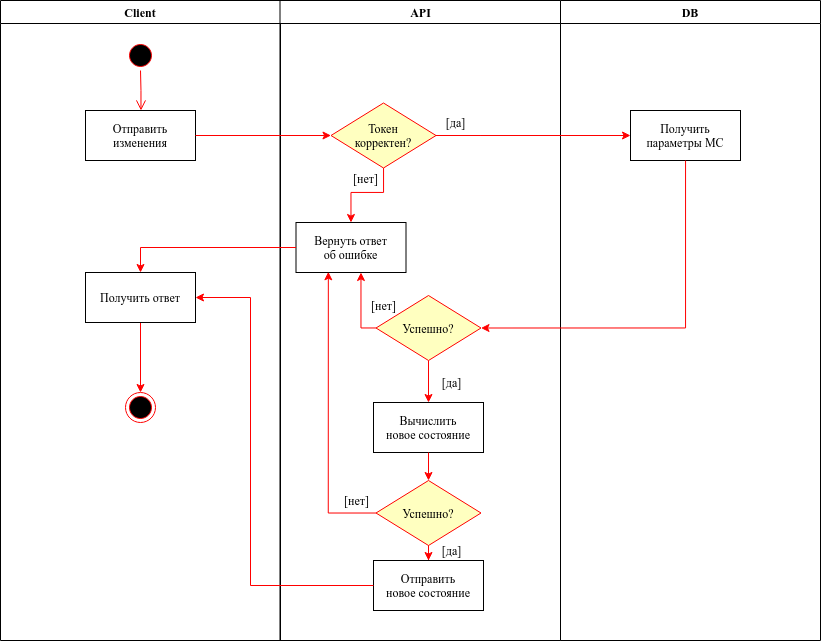
\includegraphics[width=0.7\textwidth]{diagrams/activity_send_change.png}
    \caption{Диаграмма Activity передачи изменения состояния}
    \label{fig:activity_send_change}
\end{figure}
\section*{Заключение}\label{Заключение}

В ходе данной работы были более подробно рассмотрены прецеденты, полученные
на первом этапе; были выделены слои приложения, обозначены способы взаимодейтсивя
между ними.

\end{document} % конец документа
